%!TEX root = ../thesis.tex

\section{end-to-end学習}
end-to-end学習とは, 人工ニューラルネットワークを使用して, 入力データから出力を直接
生成する方法のことを指す. \par
実世界における自動運転を例に挙げる. end-to-end学習を用いない場合, 人物や障害物などの
物体認識, 車線の検出, 経路計画, ステアリングの制御など, 多くのタスクを解決する必要が
ある. しかし, end-to-endを用いることで, 先程の
タスクを解決することなく, 車両が撮影したカメラ映像から直接, 運転操作を
行うことができる. 
% \subsection{RoboCup}
\vspace{5cm}

\begin{figure}[hbtp]
  \centering
 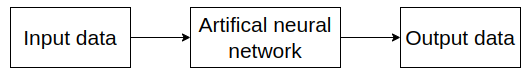
\includegraphics[keepaspectratio, scale=0.7]
      {images/end-to-end.png}
 \caption{Structure of end-to-end learning}
 \label{Fig:end-to-end}
\end{figure}

% \subsubsection{etc...}
\newpage
